\section{硬件架构}

\subsection{硬件模块层次关系}
硬件整体架构和模块层次关系,以列表方式呈现如下。在顶层模块\texttt{top.v}下,包含\texttt{CortexM0}处理器和\texttt{AHBLite}总线两个模块。总线的功能是使处理器可以同多个外设进行交互。总线模块除了包含总线控制所必须的Decoder模块和SlaveMux模块,还包含了总线上连接的各个外设模块。在列表中注意到,每个外设模块都包含了“外设的总线接口"和“外设本体”两个部分,以定时器为例,Timer模块实现了具体的定时功能,AHBLiteTimer模块则在总线和定时器模块之间传递数据,即将外设“接入”总线。
\begin{itemize}
    \ttfamily%
    \item CortexM0.v 
    \begin{itemize}
        \item cortexm0ds\_logic.v
    \end{itemize}
    \item AHBLite.v 
    \begin{itemize}
        \item AHBLiteDecoder.v 
        \item AHBLiteSlaveMux.v 
        \item AHBLiteBlockRam.v \#(.ADDR\_WIDTH(14)) [uAHBRAMCode]
        \begin{itemize}
            \item BlockRam.v  \textnormal{\small 程序空间共$2^{14}=0\mathrm{x}4000=16\mathrm{K}$字节}。
        \end{itemize}
        \item AHBLiteBlockRam.v \#(.ADDR\_WIDTH(15)) [uAHBRAMCode]
        \begin{itemize}
            \item BlockRam.v  \textnormal{\small 数据空间共$2^{15}=0\mathrm{x}8000=32\mathrm{K}$字节}。
        \end{itemize}
        \item AHBLiteGPIO.v 
        \begin{itemize}
            \item GPIO.v  \textnormal{\small 通用输入输出模块,共4个端口,每个端口可连接32个引脚。}
        \end{itemize}
        \item AHBLiteUART.v 
        \begin{itemize}
            \item UART.v  \textnormal{\small 串口通讯模块}
        \end{itemize}
        \item AHBLiteDigit.v 
        \begin{itemize}
            \item Digit.v  \textnormal{\small 数码管驱动模块,共4位。}
        \end{itemize}
        \item AHBKeyBoard.v 
        \begin{itemize}
            \item KeyBoard.v  \textnormal{\small 键盘驱动模块,共16个按键。}
        \end{itemize}
        \item AHBLiteBuzzer.v 
        \begin{itemize}
            \item Buzzer.v  \textnormal{\small 蜂鸣器驱动模块,可实现7个音阶的蜂鸣。}
        \end{itemize}
        \item AHBLiteTimer.v 
        \begin{itemize}
            \item Timer.v  \textnormal{\small 计时器模块,提供毫秒单位的系统时间。}
        \end{itemize}
        \item AHBLiteGPU.v
        \begin{itemize}
            \item GPU.v \textnormal{\small 显示与显存模块}
            \begin{itemize}
                \item SystemCrtlPLL.v \textnormal{\small 硬件锁相环,提供显示所需的时钟。}
                \item SDRAMControl.v \textnormal{\small 显存读写控制模块。}
                \item GPUHDMIEncoder.v \textnormal{\small 显示输出HDMI编码模块。}
                \item GPUDataControl.v \textnormal{\small 显示数据的处理模块。}
            \end{itemize}
        \end{itemize}
    \end{itemize}
\end{itemize}


\subsection{Cortex M0与AHBLite总线}
\xref{fig:硬件架构}描述了AHBLite总线与Cortex M0交互的核心过程。在Cortex M0端处有两路输出信号\texttt{HADDR}、\texttt{HWDATA}和一路输入信号\texttt{HRDATA},它们分别代表以下含义
\begin{itemize}
    \item 输出信号\texttt{HADDR},代表M0访问的地址。
    \item 输出信号\texttt{HWDATA},代表M0对外设的写数据。
    \item 输入信号\texttt{HRDATA},代表M0对外设的读数据。
\end{itemize}
\begin{Figure}[硬件架构]
    \includegraphics{build/Section02_01.fig.pdf}
\end{Figure}

无论M0试图访问哪一个外设寄存器,AHBLite总线会将\texttt{HWDATA}和\texttt{HADDR}传递给每一个外设模块,但是,AHBLite中有一个模块Decoder会根据地址\texttt{HADDR}判断当前M0试图访问的地址位于哪一外设中,并给出一组\texttt{HSEL}信号。外设只有在\texttt{HSEL}为高时才会工作。若为写操作,外设会将\texttt{HWDATA}的数据写入地址\texttt{HADDR}中,若为读操作,外设会将地址\texttt{HADDR}中的数据读至\texttt{HRDATA}中。每个外设都会产生一个\texttt{HRDATA}信号,但同时只有一个外设在真正工作,因此SlaveMux模块将会根据\texttt{HSEL}信号对各外设产生的\texttt{HRDATA}进行数据选择,将M0读取的那一外设给出的\texttt{HRDATA}返回给M0。

项目的M0处理器IP通过Arm官网获取,项目的AHBLite总线来自硬木课堂提供的示例程序,但在此基础上,根据项目实际做出了一些改进,主要体现为以下两点。

\subsubsection{层次化设计}
挂载于总线的外设,有两个模块组成。以内存为例,第一个模块是BlockRAM,它是内存的实现,包含了内存空间对应的BRAM资源和内存的读写操作,第二个模块则是AHBLiteBlockRAM,它是内存的总线接口,它负责将内存所需的输入输出信号与总线连接。换言之,每个外设都是由“外设本体”和“外设的总线接口”两个模块构成。

原有示例程序的架构中,如\xref{fig:原有架构}所示,外设和外设的总线接口都直接在顶层模块中实例化。作为示例,这是简便直观的。但是,作为项目工程,这种方式存在诸多问题。首先,这会将外设与外设的总线接口之间许多内部接线不必要的暴露在顶层模块中,造成代码维护上的困难。其次,若某一同类型外设需要实例化两次,仍以内存为例,我们需要程序空间RAMCode和数据空间RAMData两个实例。依这种实现方式,需要将BlockRAM和AHBLiteBlockRAM实例化两次,并重复两遍内部接线,这是不合理的。

现在经过改进的架构,如\xref{fig:现有架构}所示,坚持Verilog自顶向下的设计思想,将外设作为外设的总线接口的一个子模块,使得后者不仅仅再是一个接口,而是一个带有接口的完整外设。这样,在实例化外设时,只需要将外设的总线接口实例化即可,外设本身会作为其子模块被间接实例化,外设与外设的总线接口间的内部连线也不会暴露。对比\xref{fig:原有架构}和\xref{fig:现有架构}可以看出,创建两个同类型外设时,这种架构确实能减少重复代码。


\begin{Figure}[层次化设计优化]
    \begin{FigureSub}[原有架构]
        \includegraphics[scale=0.9]{build/Section02_02.fig.pdf}
    \end{FigureSub}\\ \vspace{0.5cm}
    \begin{FigureSub}[现有架构]
        \includegraphics[scale=0.9]{build/Section02_03.fig.pdf}
    \end{FigureSub}
\end{Figure}

\subsubsection{参数化设计}
原有示例程序的架构中,对于\texttt{HSEL}或\texttt{HRDARA}这类随着外设数量变化的信号,在编写输入输出接口时,往往是以\texttt{HSEL1}、\texttt{HSEL2}、\texttt{HSEL3}、\texttt{HSEL4}这样的方式逐个罗列的。但是,在项目实践中,常常需要向总线添加新的外设,而在原有架构中,增加外设的数量意味着需要在若干个代码文件中复制黏贴若干个与外设数量有关的信号接口。这不仅会极大的增大新增外设的工作量,还很容易因为复制黏贴中的疏漏,造成错误。

现在经过改进的架构中,则将这类与外设接口有关的信号统一以“数组”形式实现,由于Verilog中不允许在输入输出接口上使用数组,这里的“数组”实际是以位宽的方式实现的。假设有$16$个外设,原先位宽为$1$的\texttt{HSEL}则变为\texttt{HSEL\_A[16-1:0]},原先位宽为$32$的\texttt{HRDARA[31:0]}则变为\texttt{HRADATA\_A[32*16-1:0]}。并且,程序中还将这里的“外设数量16”通过宏定义的方式进行参数化,使得接口的设计无关外设数目,如果需要增加外设数目,只需要修改相应参数即可。这部分可以参见\xref{code:外设接口相关信号的参数化设计}给出的片段。

\lstinputlisting[
    style       =   Verilog,
    caption     =   {外设接口相关信号的参数化设计},
    label       =   {code:外设接口相关信号的参数化设计}
]{code/Code01.v}

参数化的设计并不仅限于此处,而是贯彻到了每一段代码中。例如,原先外设的编号和地址都是直接写在代码中的,但是,外设编号会在若干个地方出现,外设编号和地址又可能会根据需要反复调整,原先这种修改是麻烦且容易出错的,但参数化之后就解决了这个问题。这部分改动的必要性和实际效果可参见\xref{code:外设编号和地址在Decoder中的参数化}和\xref{code:外设编号在实例化时反复被使用}给出的代码片段。

\lstinputlisting[
    style       =   Verilog,
    caption     =   {外设编号在实例化时反复被使用},
    label       =   {code:外设编号在实例化时反复被使用}
]{code/Code02.v}

\lstinputlisting[
    style       =   Verilog,
    caption     =   {外设编号和地址在Decoder中的参数化},
    label       =   {code:外设编号和地址在Decoder中的参数化}
]{code/Code03.v}

目前,总线共有16个外设接口,实际启用了前12个,各外设的编号和内存地址如\xref{tab:外设的编号和内存地址}所示,程序空间和数据空间的地址分别从\texttt{0x00000000}和\texttt{0x20000000}开始,外设寄存器的内存地址则从\texttt{0x60000000}开始,每个外设递增\texttt{0x00010000}的内存地址。

\begin{Table}[外设的编号和内存地址]
<外设编号&外设名称&外设说明&外设地址&备注\\>
\texttt{00}&RAMCode&程序内存空间&\texttt{0x00000000}&共16KB空间\\
\texttt{01}&RAMData&数据内存空间&\texttt{0x20000000}&共32KB空间\\
\texttt{02}&SDRAM&SDRAM测试&\texttt{0x40000000}&已停用的测试接口\\
\texttt{03}&Timer&计时器&\texttt{0x60010000}&--\\
\texttt{04}&GPIO&通用输入输出&\texttt{0x60020000}&连接开关、LED、WII手柄\\
\texttt{05}&UART&串口通讯&\texttt{0x60030000}&--\\
\texttt{06}&IIC&WII手柄&\texttt{0x60040000}&已弃用,手柄现改挂GPIO\\
\texttt{07}&GPULite&显示控制&\texttt{0x60040000}&包含SDRAM显存和HDMI编码\\
\texttt{08}&HDMI&HDMI测试&\texttt{0x60050000}&已停用的测试接口\\
\texttt{09}&Buzzer&蜂鸣器&\texttt{0x60060000}&--\\
\texttt{10}&Digit&数码管&\texttt{0x60070000}&--\\
\texttt{11}&KeyBoard&键盘&\texttt{0x60080000}&--\\
\texttt{12}&--&--&--&未启用\\
\texttt{13}&--&--&--&未启用\\
\texttt{14}&--&--&--&未启用\\
\texttt{15}&--&--&--&未启用\\
\end{Table}

\subsection{内存模块}
内存模块包含程序空间RAMCode和数据空间RAMData两部分,硬件上两者分别分配了16KB和32KB的空间,两者均基于EG4S20片上BRAM 9K资源实现。

然而,后期由于游戏程序需要存储大量游戏地图和游戏角色的点阵数据,程序空间出现不足。为此,如\xref{fig:Keil中的相关配置}所示,在Keil中配置Memory时从数据空间末尾挪用了8KB空间(即0x2000)至程序空间,并且,在Keil中配置编译优化选项为\texttt{-Oz}空间优化,从而尽可能减小程序占用的空间体积。这两项措施有效解决了程序空间不足的问题。

\lstinputlisting[
    style       =   Verilog,
    caption     =   {内存模块的硬件代码},
    label       =   {code:内存模块的硬件代码}
]{code/Code04.v}

\begin{Figure}[Keil中的相关配置]
    \begin{FigureSub}[内存配置]
        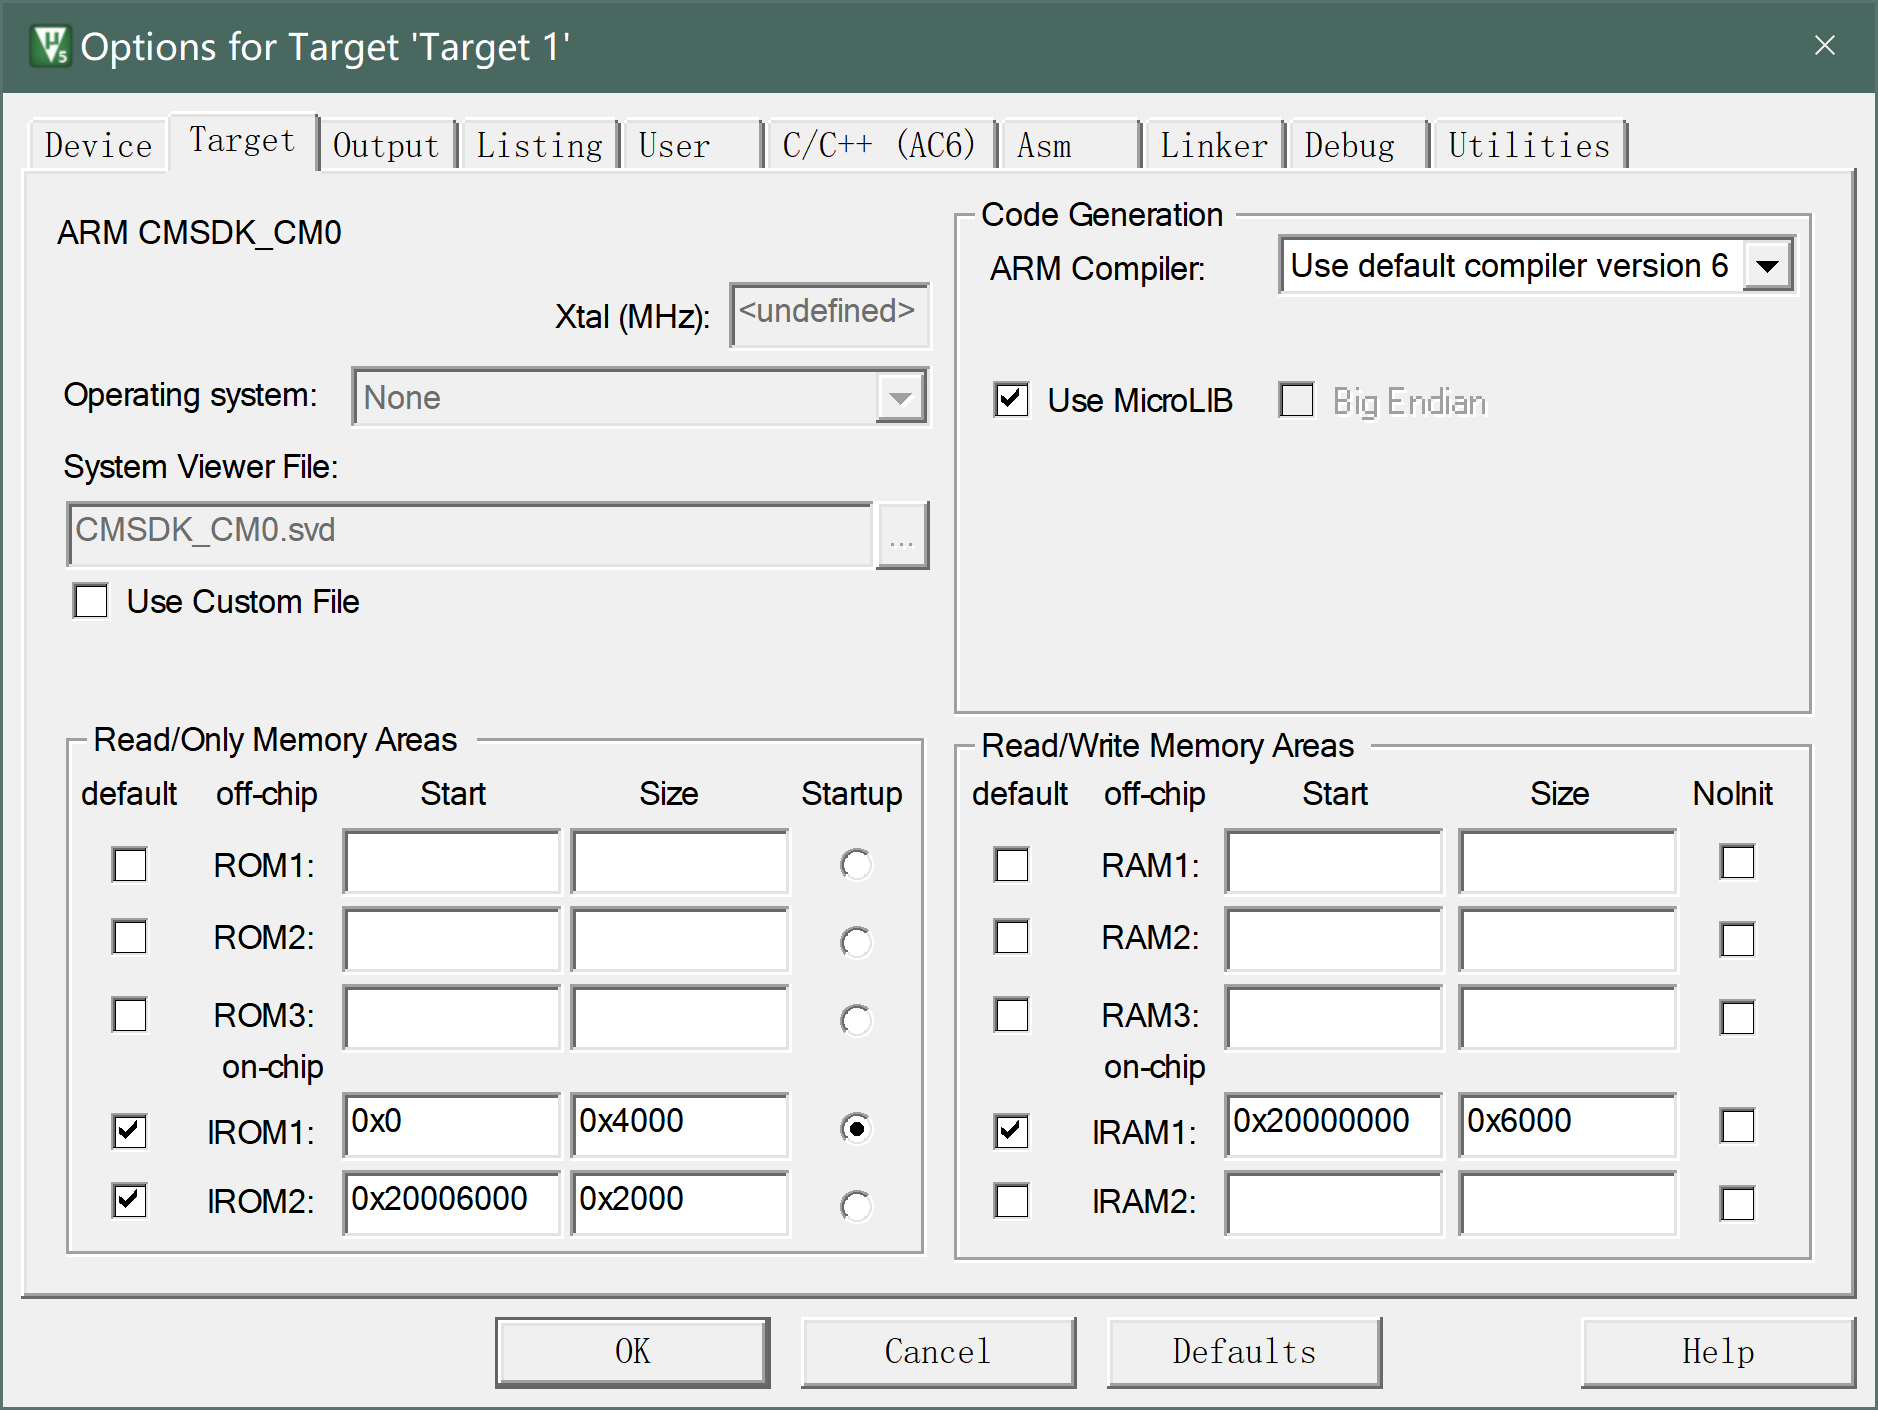
\includegraphics[width=0.4\linewidth]{image/1.png}
    \end{FigureSub}
    \hspace{0.1\linewidth}
    \begin{FigureSub}[编译优化]
        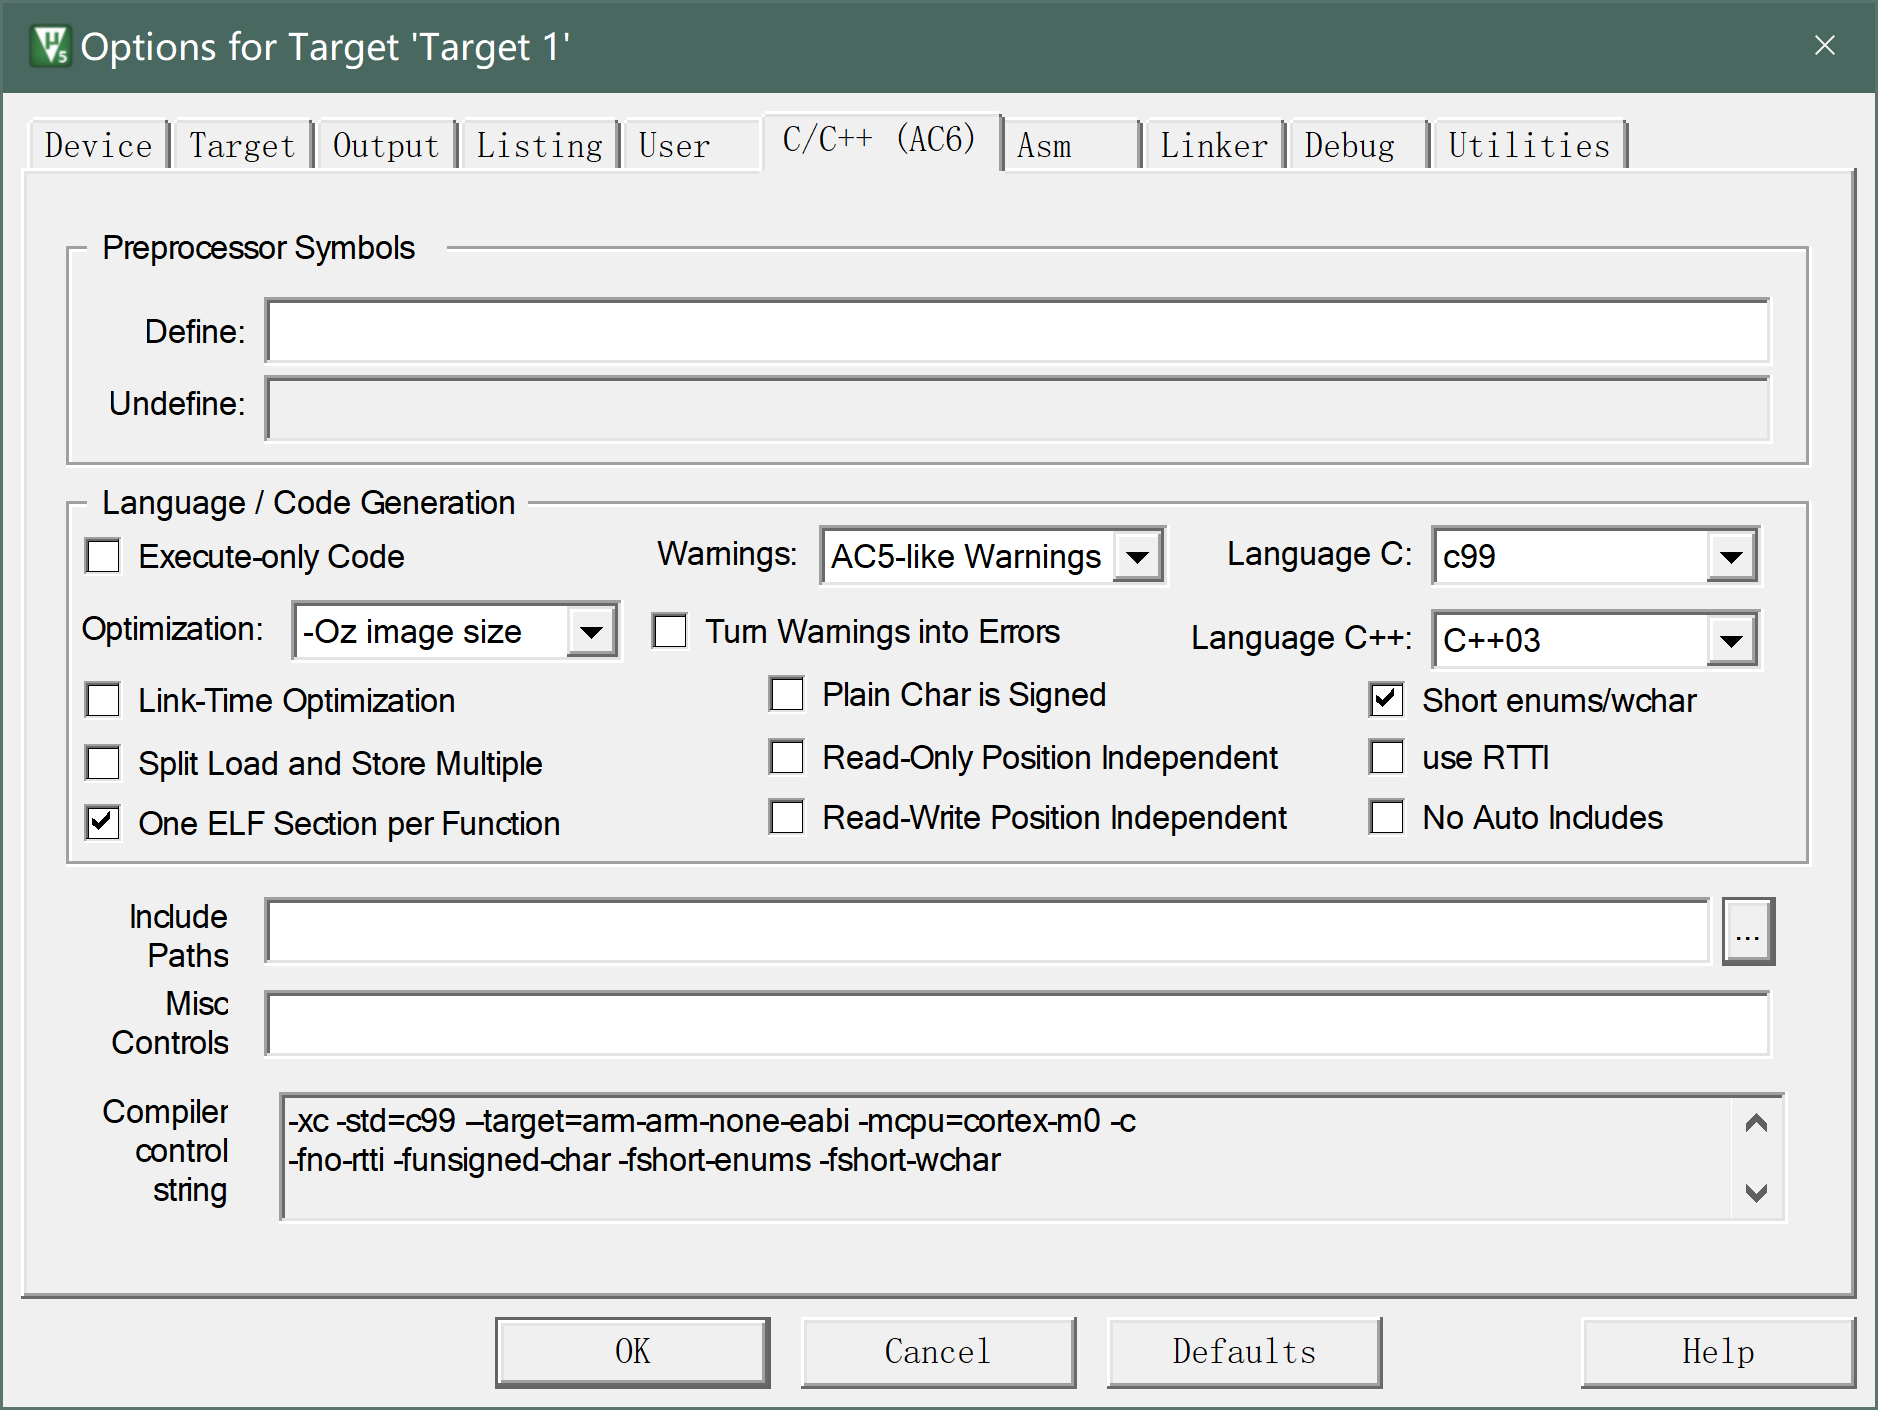
\includegraphics[width=0.4\linewidth]{image/2.png}
    \end{FigureSub}
\end{Figure}

\subsection{GPIO模块的IP设计}
GPIO即通用输入输出(General Purpose Input Output),适合用于连接一些对速度要求不高的外设。GPIO模块的实现参照了硬木课堂的示例程序,但做出了比较大的改进。首先,原有的示例程序仅支持将整组引脚设置为读模式或写模式,而改进后,可以实现对每一单引脚的读写模式选择。其次,原有的示例程序在写模式下,写出的数据是不可读回的,而改进后则为每个引脚配置了三个寄存器,如\xref{code:GPIO模块的硬件代码}所示
\begin{enumerate}
    \item \texttt{IDAT}即输入数据,其跟随引脚的输入变化。
    \item \texttt{OENA}即输出状态,其跟随来自总线的输出状态变化。若为1表示输出模式,此时会将\texttt{ODAT}输出至引脚上,若为0表示输入模式,此时会将高阻态输出至引脚上。
    \item \texttt{ODAT}即输出数据,其跟随来自总线的输出数据变化。
\end{enumerate}

GPIO模块在开发过程中曾出现过C语言中试图访问相应寄存器,但出现错误的问题。经调试,发现是C语言在编译时生成了半字(16位)或字节(8位)访问的汇编指令,而原有的硬件代码仅支持字(32位)访问。经研究,如\xref{tab:字节访问和半字访问的支持}所示,通过分析总线信号,判断当前的访问类型,确定四个字节中,哪些字节需要被访问,哪些字节不需要被访问。由此,实现了硬件对半字访问和字节访问的全面支持,解决了问题。该功能最终被封装为SizeDecoder的模块,如\xref{code:SizeDecoder模块对字节访问和半字访问的支持}所示,应用于所有外设的总线接口中。
\begin{Table}[字节访问和半字访问的支持]{lccc}
    <访问类型&\texttt{HADDR[1:0]}&\texttt{HSIZE[1:0]}&当前需要访问的字节\\>
    32位~字访问&00&10&1111\\
    \hlinelig
    \mr{2}{16位~半字访问}
    &00&01&0011\\
    &10&01&1100\\
    \hlinelig
    \mr{4}{08位~字节访问}
    &00&00&0001\\
    &01&00&0010\\
    &10&00&0100\\
    &11&00&1000\\
\end{Table}

\lstinputlisting[
    style       =   Verilog,
    caption     =   {GPIO模块的硬件代码},
    label       =   {code:GPIO模块的硬件代码}
]{code/Code05.v}

\lstinputlisting[
    style       =   Verilog,
    caption     =   {SizeDecoder模块对字节访问和半字访问的支持},
    label       =   {code:SizeDecoder模块对字节访问和半字访问的支持}
]{code/Code06.v}

GPIO模块每个端口可以连接32个引脚,硬件上共设有4个端口\texttt{PORTA}、\texttt{PORTB}、\texttt{PORTC}、\texttt{PORTD}。不过目前,实际只启用了前两个,\texttt{PORTA}的低8位和次低8位分别连接了开关和LED灯,\texttt{PORTB}的最低位和次低位则分别连接了WII手柄的IIC协议所需的SCL和SDA信号(关于WII手柄的使用和IIC协议,详见\xref{sec:智能化IP设计}中的内容)。

GPIO模块在硬件抽象层中,有着一组极为精巧的宏定义。GPIO模块每个端口的寄存器结构如\xref{code:GPIO模块的寄存器结构},诚然,当然可以直接通过结构体的方式操作引脚。但由于每个引脚仅是寄存器\texttt{I\_DAT}、\texttt{O\_ENA}、\texttt{O\_DAT}中的一位,这种操作需要使用位运算,较繁琐。

\lstinputlisting[
    style       =   C,
    caption     =   {GPIO模块的寄存器结构},
    label       =   {code:GPIO模块的寄存器结构}
]{code/Code07.c}

为了简化GPIO引脚的操作,引入了\xref{code:GPIO引脚操作符}中的一系列宏定义,首先是\xref{code:GPIO引脚操作符}中的\texttt{BASE(PORT)}和\texttt{P}、\texttt{I}、\texttt{O}、\texttt{R}、\texttt{L}、\texttt{H}、\texttt{V}七个操作符。这两者需要联用,\texttt{BASE(PORT)}的参数\texttt{PORT}即GPIO端口第一个寄存器\texttt{I\_DAT}对应的变量,先取地址\texttt{(\&(PORT))},随后再解引用\texttt{*((\&(PORT))},但解引用的右括号没有闭合。同时,也注意到七个操作符都是以\texttt{+0)}、\texttt{+1)}、\texttt{+2)}开头,将操作符置于\texttt{BASE(PORT)}后,即可闭合其解引用的右括号,同时,解引用的地址被分别偏离了$0$位、$1$位、$2$位,解引用的结果就分别是寄存器\texttt{I\_DAT}、\texttt{O\_ENA}、\texttt{O\_DAT}。七个操作符后还带有一个位运算操作,它被期望与一个仅有第\texttt{x}位为$1$的变量\texttt{BIT(x)}进行位运算,这里\texttt{x}代表操作对象是第\texttt{x}个引脚,如\xref{code:GPIO引脚定义}所示。位运算操作具体包括:读\texttt{\&}、置零\texttt{\&=\~{}}、置一\texttt{|=}、翻转\texttt{\^{}=},共计有四种。

\lstinputlisting[
    style       =   C,
    caption     =   {GPIO引脚操作符},
    label       =   {code:GPIO引脚操作符}
]{code/Code08.c}

\lstinputlisting[
    style       =   C,
    caption     =   {GPIO引脚定义},
    label       =   {code:GPIO引脚定义}
]{code/Code09.c}

由此,只要依照引脚端口\texttt{BASE(PORT)}、引脚待定操作符\texttt{X}、引脚位置\texttt{BIT(x)}的顺序排列宏定义,如\xref{code:GPIO引脚定义}所示,就可以将每个引脚的操作从形式上做成一个函数,形如\texttt{LED\_0(X)}或\texttt{SWI\_0(X)},其中\texttt{X}可以是七个操作符中的一个,取决于传入哪一操作符,就可以实现对三个寄存器中相应位的不同读写操作,实现对引脚状态的控制。在\xref{code:GPIO宏定义的示例}中,给出了这方面的一个示例,可以看出,经过上述宏定义的封装,引脚的控制变得极为简洁优雅,且具有整齐统一的操作方法。其背后复杂的位运算过程被隐藏。

\lstinputlisting[
    style       =   C,
    caption     =   {GPIO宏定义的示例},
    label       =   {code:GPIO宏定义的示例}
]{code/Code10.c}

\subsection{UART模块的IP设计}
UART即通用异步收发器(Universal Asynchronous Receiver/Transmitter),在项目中其被用于串口通讯,使系统可以通过串口输出调试信息。UART模块的寄存器在硬件抽象层被封装为了如\xref{code:UART模块的寄存器结构}所示的结构体,并同时定义了如\xref{code:UART模块的函数}所示的函数进行字符的读写操作。另外,在复赛期间,进一步实现了字符串格式化输出,基于此,自行定义了\texttt{<stdio.h>}风格的\texttt{printf()}函数,这极大地便利了调试信息的串口输出。

\lstinputlisting[
    style       =   C,
    caption     =   {UART模块的寄存器结构},
    label       =   {code:UART模块的寄存器结构}
]{code/Code11.c}

\lstinputlisting[
    style       =   C,
    caption     =   {UART模块的函数},
    label       =   {code:UART模块的函数}
]{code/Code12.c}

\subsection{Timer模块的IP设计}
Timer模块实现了定时器功能.硬件上设一个32位的寄存器,通过对时钟信号分频,使寄存器的数值每隔$1$毫秒加$1$,从而可以提供一个毫秒精度的系统时间,经计算,这可以提供近50天的连续计时,完全能满足系统需要。Timer模块的寄存器结构如\xref{code:Timer模块的寄存器结构}所示。在项目实践中,定时器主要用于稳定帧长,由于在游戏中,取决于画面的复杂程度,每一帧绘制的时长是不一样的,这就可能导致游戏画面时快时慢,造成不稳定的游戏体验。通过Timer模块,在每一帧开始时记录一个时间\texttt{nowTime},事先测量该画面最大帧长并保存在宏定义\texttt{FRAME}中,作为帧长,在每一帧的任务结束后,等待至系统时间大于帧开始时记录的时间\texttt{nowTime}加上帧长\texttt{FRAME},达到稳定帧长的目的。

\lstinputlisting[
    style       =   C,
    caption     =   {Timer模块的寄存器结构},
    label       =   {code:Timer模块的寄存器结构}
]{code/Code13.c}

\lstinputlisting[
    style       =   C,
    caption     =   {Timer模块的使用实例},
    label       =   {code:Timer模块的使用实例}
]{code/Code14.c}

\subsection{Buzzer模块的IP设计}
Buzzer模块是蜂鸣器的驱动模块。板卡上搭载的蜂鸣器是无源蜂鸣器,其驱动方式如下,即若要令蜂鸣器产生$f\;\si{Hz}$的声音,则需要向蜂鸣器的引脚输出$f\;\si{Hz}$的电信号,由此可见,Buzzer模块实际就是一个分频器。Buzzer模块的寄存器结构如\xref{code:Buzzer模块的寄存器结构}所示。其中,寄存器\texttt{NOTE}可以通过写$1,2,3,4,5,6,7$指定音阶,对应Do、Re、Me、Fa、So、La、Si,其频率已被内置在硬件中。寄存器\texttt{TIME}则可以指定音长,单位是毫秒。Buzzer模块在\texttt{TIME}非零时产生\texttt{NOTE}对应频率的蜂鸣,并将\texttt{TIME}每毫秒减去$1$。
\lstinputlisting[
    style       =   C,
    caption     =   {Buzzer模块的寄存器结构},
    label       =   {code:Buzzer模块的寄存器结构}
]{code/Code15.c}

\subsection{KeyBoard模块的IP设计}
KeyBoard模块是矩阵键盘的驱动模块。键盘为$4\times 4$,共有16个按键,其通过扫描方式工作。KeyBoard模块的寄存器结构如\xref{code:KeyBoard模块的寄存器结构}所示,当有按键按下时,\texttt{KEY}中的值相应为\texttt{0x00}、\texttt{0x01}、\texttt{0x02}、……、\texttt{0x0F},当没有按键按下时,\texttt{KEY}中的值则为\texttt{0xFF}。

\lstinputlisting[
    style       =   C,
    caption     =   {KeyBoard模块的寄存器结构},
    label       =   {code:KeyBoard模块的寄存器结构}
]{code/Code16.c}

\subsection{Digit模块的IP设计}
Digit模块是四位数码管的驱动模块,其寄存器结构如\xref{code:Digit模块的寄存器结构}所示。\texttt{DIG}可以作为数组\texttt{DIG[0] DIG[1] DIG[2] DIG[3]}使用,分别对应四个数码管的状态。在结构体成员中,\texttt{COD}为数码管显示数码,取值范围为\texttt{0x0}至\texttt{0xF}。\texttt{DOT}控制数码管附带的小数点是否点亮。\texttt{ENA}控制数码管的使能,为$0$时将该数码管被熄灭。\texttt{DIG\_CRTL}则控制数码管的工作方式,初始化时应将\texttt{DIG\_CRTL}赋值为\texttt{0xFF}使数码管进入扫描工作状态。

\lstinputlisting[
    style       =   C,
    caption     =   {Digit模块的寄存器结构},
    label       =   {code:Digit模块的寄存器结构}
]{code/Code17.c}

\subsection{GPULite模块的IP设计}
GPULite模块实现了系统的显示功能,使用SDRAM作为显存,使用HDMI作为图像输出。模块实现了M0对显示屏的的完全控制,即M0可以控制显示屏上每一个像素点的颜色(而不是只能显示一些硬件预设的图形)。并且,经过优化后,模块可以保持一个合理的刷新速率,模块可以做到无闪烁的显示,从而提供一个较好的显示体验。

GPULite模块主要分为三部分
\begin{enumerate}
    \item 片上SDRAM资源的读写封装。
    \item 显存的写入,将M0提供的绘图数据存入显存中。
    \item 显存的读取,将显存的数据读出,并依照VESA时序经HDMI编码后输出。
\end{enumerate}

\subsubsection{HDMI协议的实现}
HDMI部分参照了 \url{www.fpga4fun.com}中的一段示例代码\footnote{\url{https://www.fpga4fun.com/HDMI.html}},但作出了相当程度的修改。首先,项目使用的显示屏的分辨率为$1024\times 600$,这不是一个标准的VESA分辨率,为此,在充分理解VESA时序后,重新测试了一组可以适用于$1024\times 600$分辨率的VESA时序参数,如\xref{tab:VESA时序参数}所示。其次,示例代码原有的VESA时序存在一定的问题,在该项目中无法正常工作。调整了各显示阶段DISP、FRONT、SYNC、BACK间的先后顺序后,问题得到解决。该模块非常简洁的实现了VESA时序和HDMI编码。

\begin{Table}[适用于$1024\times 600$分辨率的VESA时序参数;VESA时序参数]{lrlr}
    <横向参量&数值&纵向参量&数值\\>
    \texttt{H\_FRONT}&24&
    \texttt{V\_FRONT}&3\\
    \texttt{H\_SYNC}&136&  
    \texttt{V\_SYNC}&6\\ 
    \texttt{H\_BACK}&160&
    \texttt{V\_BACK}&29\\  
    \texttt{H\_DISP}&1024&
    \texttt{V\_DISP}&600\\  
    \texttt{H\_TOTAL}&1344&
    \texttt{V\_TOTAL}&638\\           
\end{Table}

HDMI模块的实现充分运用了安路科技提供的IP资源。由于HDMI在物理接口上采用1:10的速度传输,因此需要两路时钟信号,一路是像素时钟,HDMI将以该频率传输像素点,一路是像素时钟的十倍频,HDMI将以该频率传输像素点中每一位的比特。然而十倍频后所需的时钟频率已经高达500MHz,经过测试FPGA在该频率下的工作出现不稳定。安路科技提供的\texttt{EG\_LOGIC\_ODDR}的IP可以将信号在输出引脚上倍频,这样就只需要输入250MHz的五倍频时钟了。安路科技提供的\texttt{EG\_PHY\_PLL}锁相环IP可以运用片上的硬件锁相环资源,产生所需50MHz和250MHz的五倍频时钟。

\lstinputlisting[
    style       =   Verilog,
    caption     =   {HDMI编码},
    label       =   {code:HDMI编码}
]{code/Code18.v}


\subsubsection{Ping Pong双缓存机制}
显示部分最初遇到的一个较明显的问题是,在刷新画面的过程中,显示会出现闪烁的现象,这严重影响了显示体验。经过研究,显示出现闪烁的原因在于向显存写入图像的过程中,HDMI从显存中读取到了半截的图像。为了解决该问题,引入了Ping Pong的双缓存机制。具体而言,这需要在SDRAM中创建两块显存空间
\begin{enumerate}
    \item 第一个周期中,M0向显存1写入,HDMI从显存2读取。
    \item 第二个周期中,M0向显存2写入,HDMI从显存1读取。
\end{enumerate}

这样,读写交替在两块显存空间进行,从而保证HDMI显示的画面始终是完整的。但是一个重要细节在于何时进行切换,当M0完成一帧的绘制发出Ping Pong指令后,硬件其实并不是立即执行Ping Pong操作,而是需要等待HDMI进入消隐间隔后再执行Ping Pong操作,以避免影响HDMI当前帧的显示。否则仍然会存在短暂的闪烁。

\subsubsection{GPULite的硬件抽象层设计}

GPULite模块的寄存器结构如\xref{code:GPULite的寄存器结构}所示,\texttt{X\_POS}和\texttt{Y\_POS}分别代表写入起始点的像素位置,\texttt{PIXEL}代表写入像素的颜色,\texttt{LEN}代表写入的长度,应指出显存是线性存储的,即当行没有写完的像素点会自动折至下一行。\texttt{ENABLE}置为$1$时模块将开始写显存,完成后应当置回$0$。\texttt{BUSY}指示模块是否正在写显存。\texttt{PING\_PONG}则是控制Ping Pong操作的寄存器。\xref{code:GPULite的基础函数}中的三个函数是对上述寄存器操作的封装,\texttt{WaitRamReady()}应当在初始化时调用,\texttt{PingPong()}用于切换Ping Pong状态,\texttt{RamWrite()}用于发出写显存指令。\xref{code:GPULite的基本绘图函数}则事先了若干基本绘图函数,包括绘制背景、绘制矩形、绘制像素。
\lstinputlisting[
    style       =   C,
    caption     =   {GPULite的寄存器结构},
    label       =   {code:GPULite的寄存器结构}
]{code/Code19.c}

\lstinputlisting[
    style       =   C,
    caption     =   {GPULite的基础函数},
    label       =   {code:GPULite的基础函数}
]{code/Code20.c}

\lstinputlisting[
    style       =   C,
    caption     =   {GPULite的基本绘图函数},
    label       =   {code:GPULite的基本绘图函数}
]{code/Code21.c}

在复赛期间,为了实现字符显示,新增了一系列软硬件代码,如\xref{code:GPULite的字符绘图函数}所示。在\xref{code:GPULite的寄存器结构}中,若将\texttt{ENABLE}置为$3$而不是$1$,则写入时,将不再是写入\texttt{PIXEL}提供的固定颜色像素,而将逐个写入\texttt{GPU\_PIXELS}数组中的像素,硬件为此做了相应的准备,这样就可以较高效的写一排颜色不同的像素了。\xref{code:GPULite的字符绘图函数}中,\texttt{LCDPixels()}是对上述过程的封装,\texttt{LCDChar()}提供了一个显示字符的函数,基于$8\times 16$点阵字体,但可以通过参数进行字体缩放。\texttt{LCDPrintf()}则在前者基础上,进一步实现了字符串的格式化输出。

\lstinputlisting[
    style       =   C,
    caption     =   {GPULite的字符绘图函数},
    label       =   {code:GPULite的字符绘图函数}
]{code/Code22.c}
